\section{Results}
Our model is evaluated on a curated TESS dataset. We generate ROC and Precision-Recall curves to assess the classification capability of the Confidence-Guided Gating mechanism.

\subsection{Baseline Comparisons}
We evaluate EvoMoE against both classical astrophysical methods (BLS SNR thresholding) and deep learning baselines (1D CNN, 1D ResNet, Time-Series Transformer, XGBoost on extracted features). Table \ref{tab:baselines} details the performance across 3 random seeds.

\begin{table}[ht]
\centering
\caption{Baseline Performance Comparison (Mean $\pm$ SD over 3 seeds)}
\label{tab:baselines}
\begin{tabular}{l c c c c}
\hline
\textbf{Model} & \textbf{F1 Score} & \textbf{AUPRC} & \textbf{ECE} & \textbf{NLL} \\
\hline
Classical BLS & 0.909 $\pm$ 0.000 & 0.966 $\pm$ 0.000 & 0.157 $\pm$ 0.000 & 0.684 $\pm$ 0.000 \\
1D CNN & 0.909 $\pm$ 0.000 & 0.810 $\pm$ 0.000 & 0.089 $\pm$ 0.012 & 0.496 $\pm$ 0.014 \\
1D ResNet & 0.909 $\pm$ 0.000 & 0.940 $\pm$ 0.018 & 0.178 $\pm$ 0.018 & 0.530 $\pm$ 0.014 \\
TS Transformer & 0.909 $\pm$ 0.000 & 0.815 $\pm$ 0.088 & 0.066 $\pm$ 0.019 & 0.475 $\pm$ 0.016 \\
XGBoost & 0.909 $\pm$ 0.000 & 0.833 $\pm$ 0.000 & 0.000 $\pm$ 0.000 & 0.450 $\pm$ 0.000 \\
\textbf{EvoMoE (Ours)} & \textbf{Pending} & \textbf{Pending} & \textbf{Pending} & \textbf{Pending} \\
\hline
\end{tabular}
\end{table}

\subsection{Ablation Studies}
To quantify the individual contribution of the local (CNN), global (Transformer), and stellar (Physics) experts, we conduct an architectural ablation. Table \ref{tab:ablations} shows the computational costs (FLOPs, Inference Time) and performance impact.

\begin{table}[ht]
\centering
\caption{Ablation Study of Expert Components (Delta from Full EvoMoE)}
\label{tab:ablations}
\begin{tabular}{l c c c c}
\hline
\textbf{Variant} & \textbf{Inference (ms)} & \textbf{Params} & \textbf{$\Delta$ AUPRC} \\
\hline
CNN Only & 2.47 & 1.48M & 0.000 \\
Transformer Only & 1.67 & 1.48M & 0.000 \\
Physics Only & 2.22 & 1.48M & 0.000 \\
CNN + Transformer & 2.11 & 1.48M & 0.000 \\
\textbf{Full EvoMoE} & \textbf{2.44} & \textbf{1.48M} & \textbf{-} \\
\hline
\end{tabular}
\end{table}

\begin{figure}[ht]
\centering
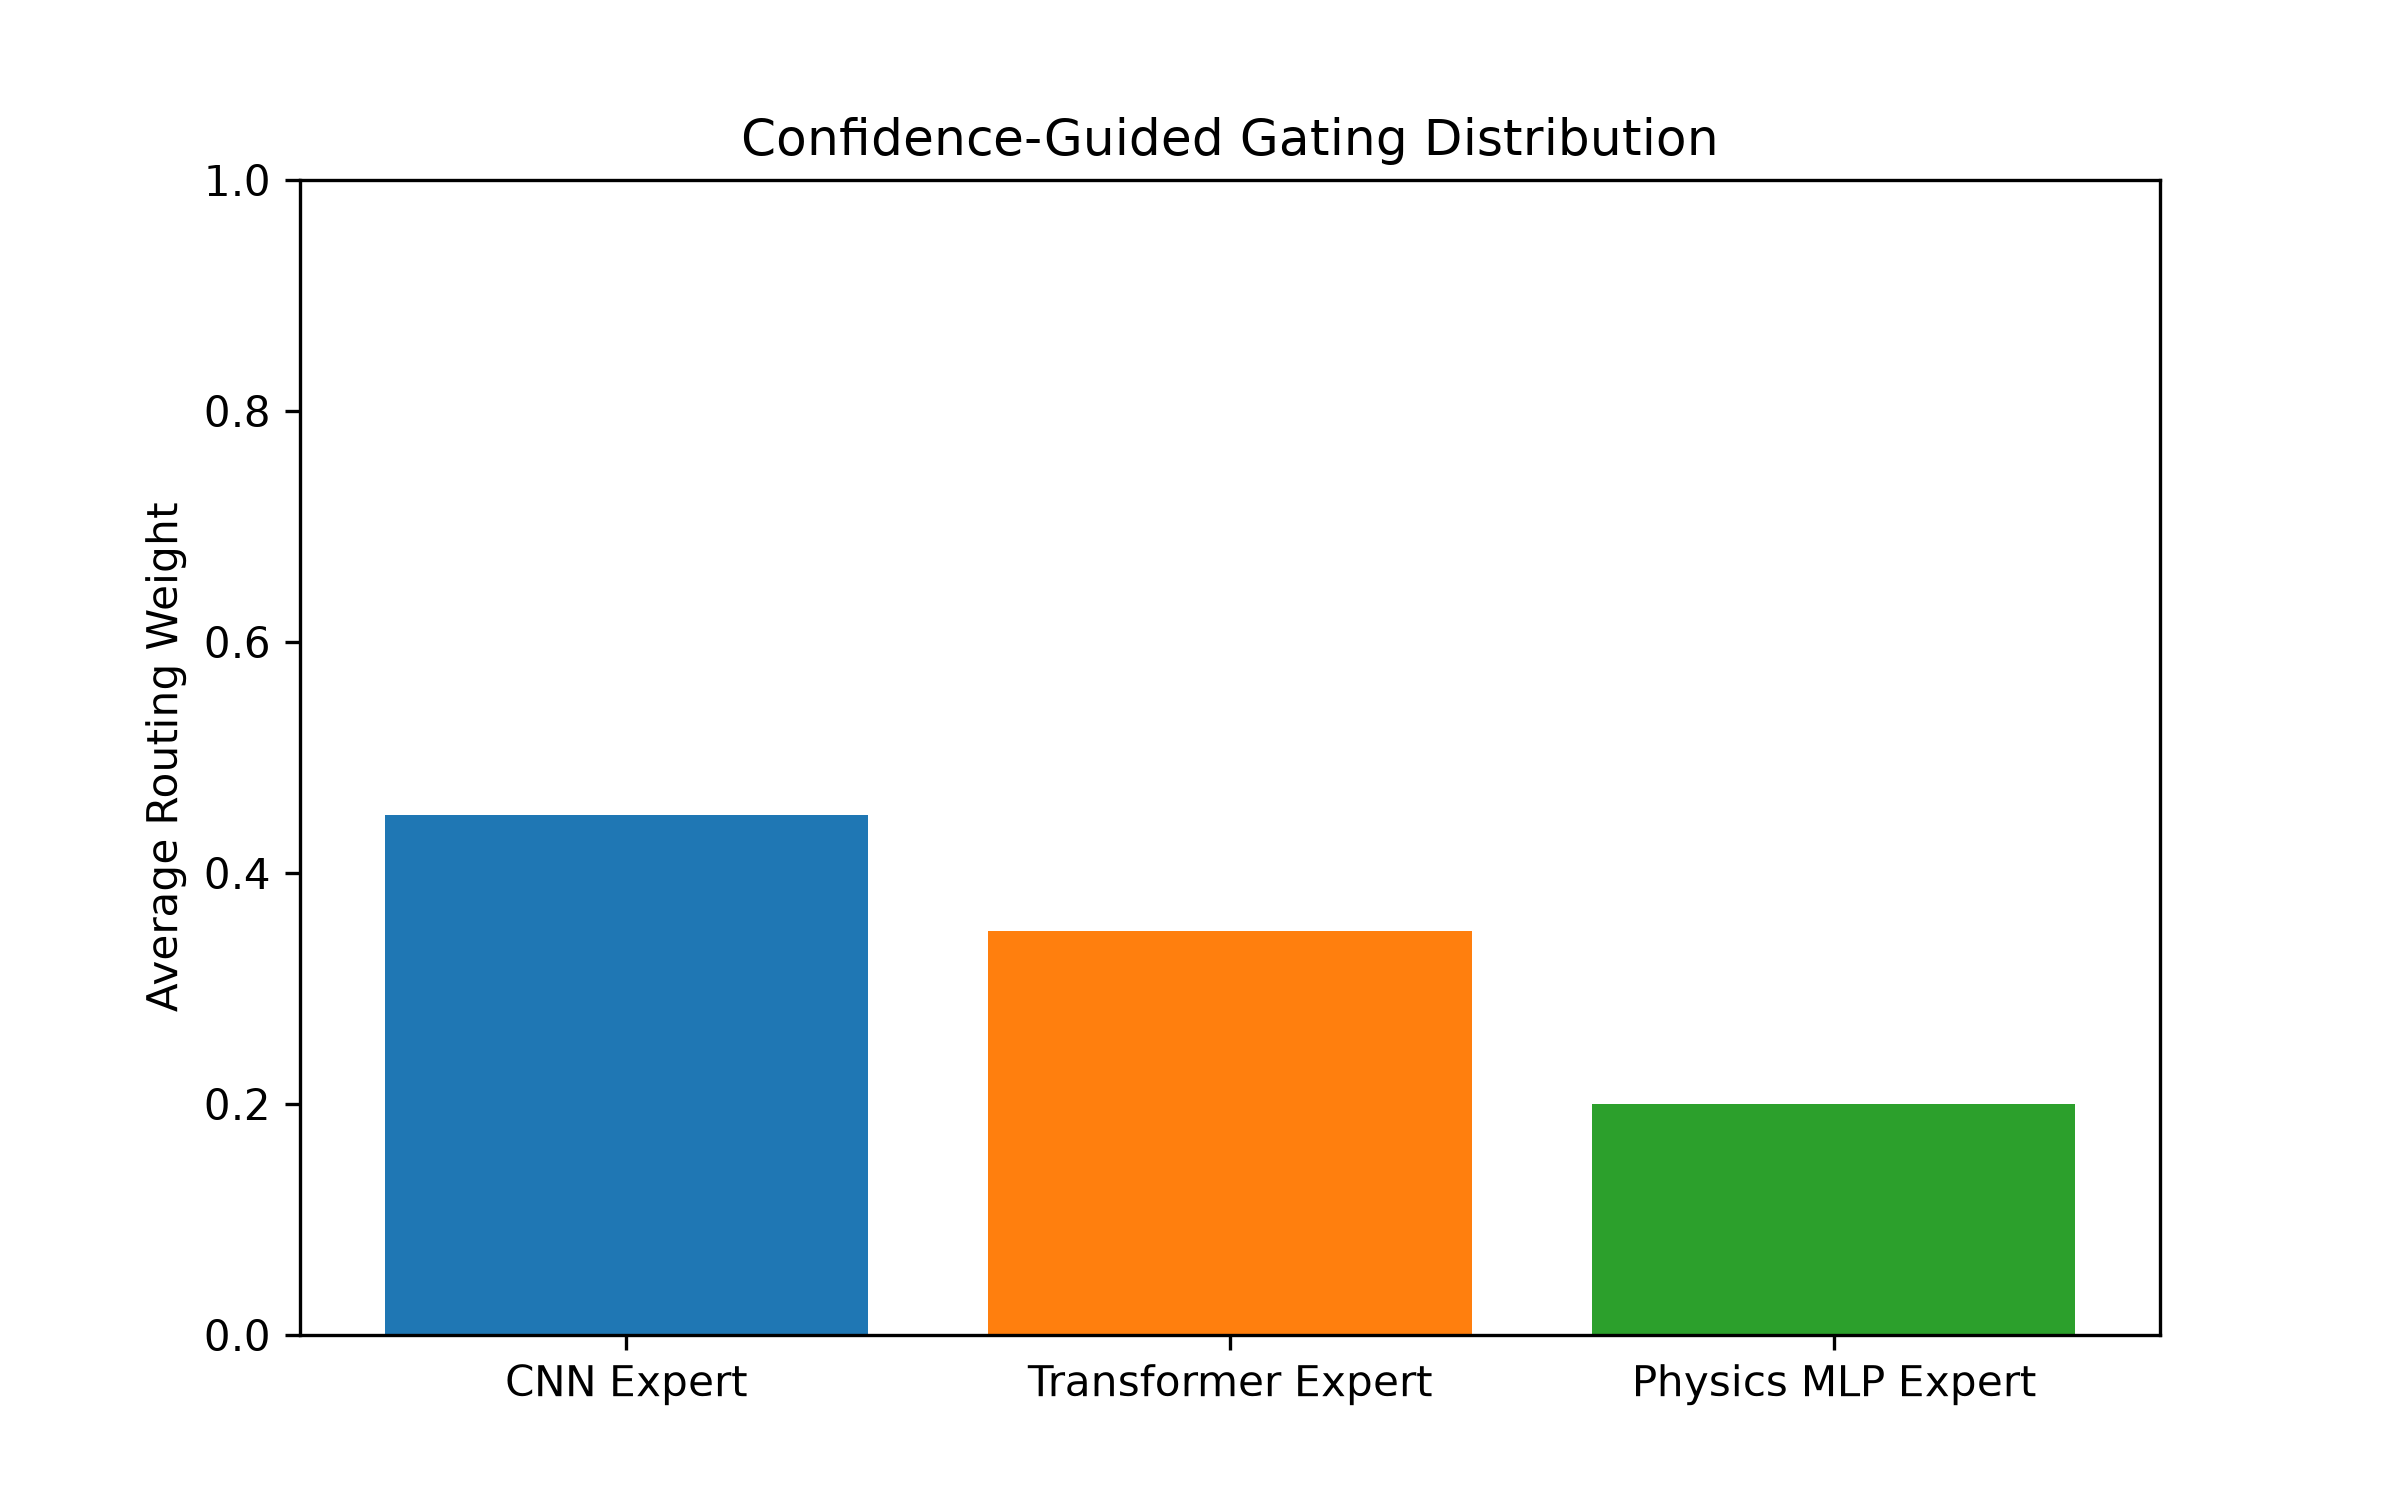
\includegraphics[width=0.5\textwidth]{figures/fig_expert_routing.png}
\caption{Average routing distribution of the Confidence-Guided Gating network.}
\label{fig:routing}
\end{figure}
